%
% $RCSfile: model_view_controller.tex,v $
%
% Copyright (c) 2001-2004. Christian Heller. All rights reserved.
%
% No copying, altering, distribution or any other actions concerning this
% document, except after explicit permission by the author!
% At some later point in time, this document is planned to be put under
% the GNU FDL license. For now, _everything_ is _restricted_ by the author.
%
% http://www.cybop.net
% - Cybernetics Oriented Programming -
%
% http://www.resmedicinae.org
% - Information in Medicine -
%
% @author Christian Heller <christian.heller@tuxtax.de>
%

\subsection{Model View Controller}
\label{model_view_controller_heading}

After having had a closer look at common design patterns for persistence and
communication, this section finally considers the so called \emph{Frontend} of
an application which is mostly realized in form of a graphical user interface.\\
Nowadays, the well-known \emph{Model View Controller} pattern (figure
\ref{model_view_controller_figure}) is used by nearly all standard applications.
Its principle is to have the \emph{Model} holding domain data, the \emph{View}
accessing and displaying these data and the \emph{Controller} providing the
workflow of the application by handling any signals (events/ actions) appearing
on the view.

\begin{figure}[ht]
    \begin{center}
       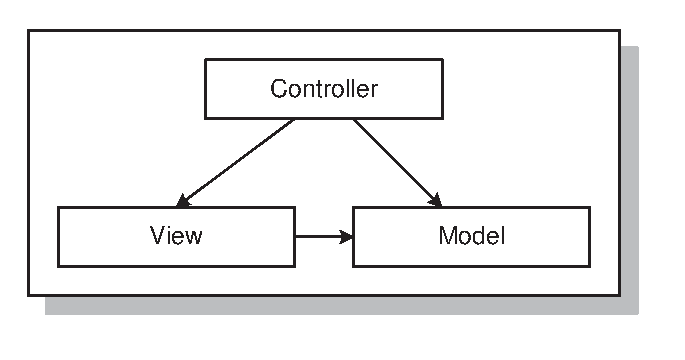
\includegraphics[scale=0.7]{vector/model_view_controller.eps}
       \caption{Model View Controller Design Pattern}
       \label{model_view_controller_figure}
    \end{center}
\end{figure}

Since the view (graphical user interface) serves as means of communication between
a software system (application) and its user (Human Being as system), the view
is in fact just another type of communication model that should be assembled
by a special translator.\\
Because there are many ways in which domain data can be displayed, different
user interfaces can exist. Each of them has to have its very own translator item
that knows how to map data both ways, from the domain model to the user interface
model and vice-versa.

